\item \textbf{ACTIVIDAD: Diseño de un sistema óptico para retina superior e inferior.}
Su grupo está entrenando para convertirse en asistentes de óptica. El técnico óptico que lo está entrenando quiere que diseñe un dispositivo que creará dos imágenes en la misma posición en el espacio, una vertical y la otra invertida. Cuando el paciente mire dentro del dispositivo, verá ambas imágenes y hará comentarios sobre su color, forma y brillo relativos. Esto le permitirá al técnico llegar a algunas conclusiones sobre las diferencias en la visión entre las partes superior e inferior de la retina. La figura TP35.2 muestra el sistema óptico, junto con el objeto único y dos imágenes. El técnico tiene una lente con una distancia focal de lente $f_{\text{Lente}} = 10.0\text{ cm}$. Él quiere que usted determine la distancia focal del espejo que necesita, dado que tiene una carcasa en la que puede montar el espejo a una distancia de $d = 40.0\text{ cm}$ de la lente. Trabaje en su grupo para analizar y proporcionar estas cantidades.

\begin{center}
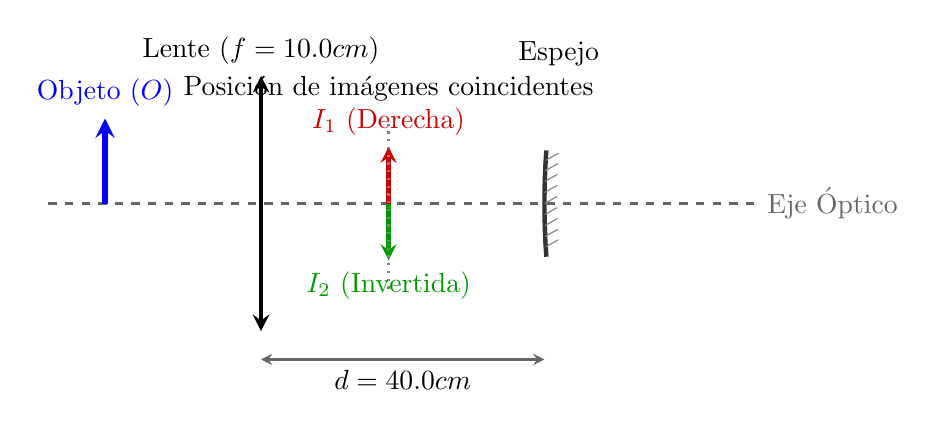
\begin{tikzpicture}[scale=0.9, >=stealth, thick]
    % Eje Óptico
    \draw[dashed, black!60] (-3,0) -- (7,0) node[right] {Eje Óptico};
    
    % Lente delgada convergente en x = 0
    \draw[ultra thick, <->] (0,-1.8) -- (0,1.8) node[above] {Lente ($f = 10.0\text{ cm}$)};
    
    % Espejo en x = 4 (distancia d = 40.0 cm)
    \draw[ultra thick, black!80, domain=-30:30] plot ({4.2 - 0.2*cos(\x)}, {1.5*sin(\x)});
    % Rayitas detrás del espejo para indicar que es espejo
    \foreach \y in {-4,-3,-2,-1,0,1,2,3,4} {
        \draw[gray, thin] ({4.2 - 0.2*cos(6*\y)}, {1.5*sin(6*\y)}) -- ({4.38 - 0.2*cos(6*\y)}, {1.5*sin(6*\y) + 0.1});
    }
    \node at (4.2, 1.8) [above] {Espejo};
    
    % Distancia d = 40.0 cm
    \draw[<->, black!60] (0,-2.2) -- (4,-2.2);
    \node at (2, -2.2) [below] {$d = 40.0\text{ cm}$};
    
    % Objeto único
    \draw[->, ultra thick, blue, line width=2pt] (-2.2,0) -- (-2.2,1.2) node[above] {Objeto ($O$)};
    
    % Las dos imágenes en la misma posición (vertical e invertida)
    \draw[->, ultra thick, red!80!black, line width=1.5pt] (1.8,0) -- (1.8,0.8) node[above] {$I_1$ (Derecha)};
    \draw[->, ultra thick, green!60!black, line width=1.5pt] (1.8,0) -- (1.8,-0.8) node[below] {$I_2$ (Invertida)};
    
    % Cota de posición de las imágenes
    \draw[dotted, gray] (1.8,-1.2) -- (1.8, 1.2);
    \node at (1.8, 1.3) [above] {Posición de imágenes coincidentes};
\end{tikzpicture}
\end{center}